\documentclass[margin=5mm]{standalone}
\usepackage[dvipsnames]{xcolor}
\usepackage{pgfplots}
\usepackage{tikz}
\usepackage[tikz]{ocgx2}

\pgfplotsset{compat=1.18}
\begin{document}

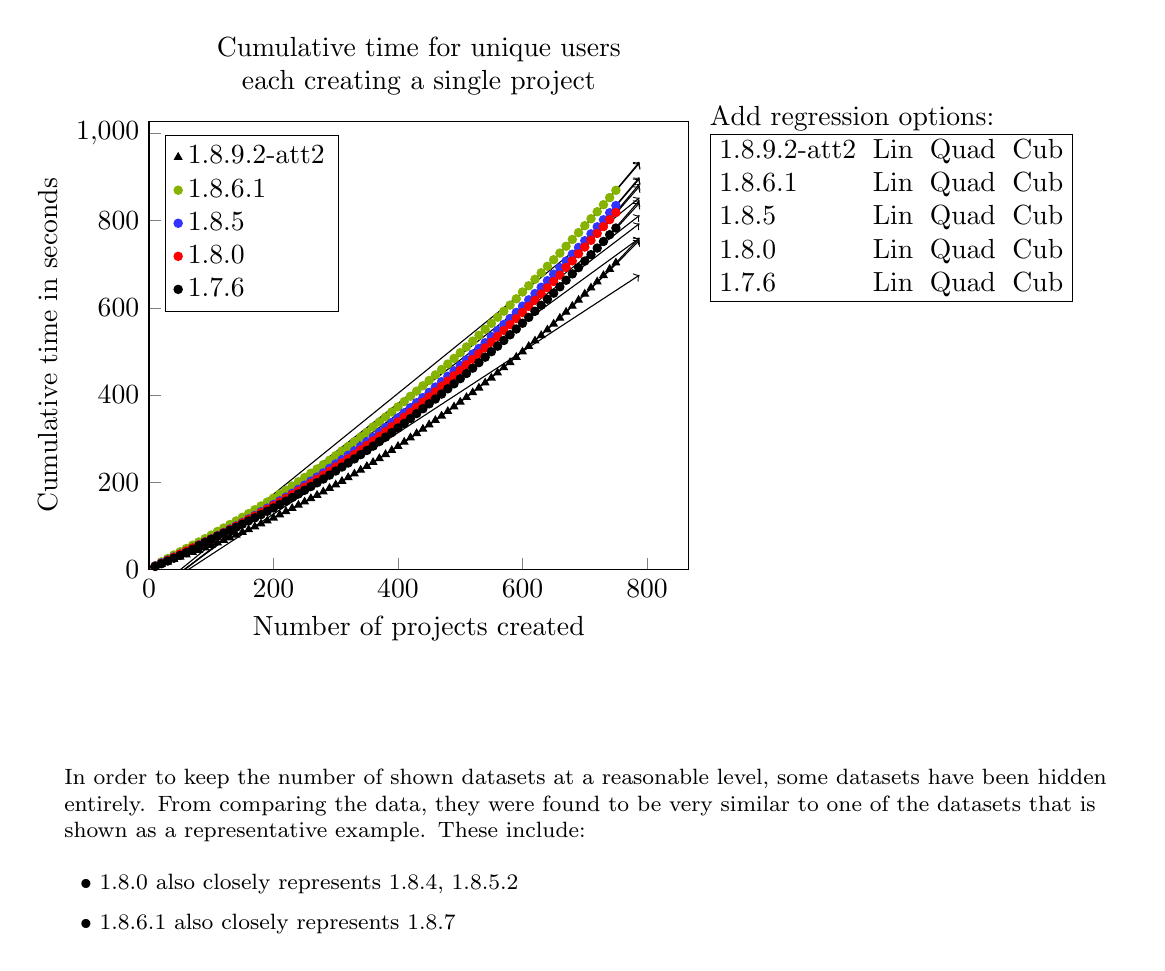
\begin{tikzpicture}
    \begin{axis}[
        align = center,
        legend pos = north west,
        legend cell align = left,
        xlabel = Number of projects created,
        ylabel = Cumulative time in seconds,
        xtick pos = left,
        ytick pos = left,
        scaled ticks = false,
        xmin = 0,
        ymin = 0,
        title = {Cumulative time for unique users each creating a single project},
        title style = {text width = 0.8\textwidth},
        legend entries={\switchocg{1.8.9.2-att2}{1.8.9.2-att2},\switchocg{1.8.6.1}{1.8.6.1},\switchocg{1.8.5}{1.8.5},\switchocg{1.8.0}{1.8.0},\switchocg{1.7.6}{1.7.6}}]
        \begin{scope}[ocg = {ref = 1.8.9.2-att2-Lin, status = invisible}]
            \plot[domain=0:788,->,forget plot] (\x,{-59.32505333333330099776503629982471466064453125 + 0.9321936842105262854829561547376215457916259765625*(\x)^1});
        \end{scope}
        \begin{scope}[ocg = {ref = 1.8.9.2-att2-Quad, status = invisible}]
            \plot[domain=0:788,->,forget plot] (\x,{5.98714693817098453365588284214027225971221923828125 + 0.423267448328674300572771471706801094114780426025390625*(\x)^1 + 0.00066963978405506856782236635439176097861491143703460693359375*(\x)^2});
        \end{scope}
        \begin{scope}[ocg = {ref = 1.8.9.2-att2-Cub, status = invisible}]
            \plot[domain=0:788,->,forget plot] (\x,{2.2876900456621225288245113915763795375823974609375 + 0.479815835534479984136879693323862738907337188720703125*(\x)^1 + 0.0004848517274861911439086392672237479928298853337764739990234375*(\x)^2 + 0.000000162094786463927635887063744175862201046811605920083820819854736328125*(\x)^3});
        \end{scope}
        \begin{scope}[ocg = {ref = 1.8.9.2-att2, status = visible}]
            \addplot[
                only marks,
                color = black,
                mark = triangle*,
                mark size = 1.5 pt
            ]coordinates {(10,6.226)(20,11.752)(30,17.29)(40,23.045)(50,28.211)(60,33.661)(70,39.258)(80,44.235)(90,49.775)(100,55.407)(110,61.142)(120,66.847)(130,72.614)(140,79.138)(150,85.418)(160,91.543)(170,97.994)(180,104.614)(190,111.36)(200,118.152)(210,125.536)(220,132.769)(230,140.211)(240,147.684)(250,155.073)(260,162.8)(270,170.409)(280,178.045)(290,186.237)(300,194.256)(310,202.463)(320,210.769)(330,219.25)(340,227.963)(350,236.5)(360,245.535)(370,254.513)(380,263.82)(390,273.164)(400,282.606)(410,292.153)(420,302.117)(430,311.934)(440,321.979)(450,331.975)(460,342.056)(470,352.115)(480,362.599)(490,373.192)(500,383.938)(510,394.655)(520,405.551)(530,416.388)(540,427.981)(550,439.248)(560,450.862)(570,462.886)(580,474.784)(590,486.859)(600,499.263)(610,511.79)(620,524.303)(630,536.668)(640,549.662)(650,563.133)(660,576.522)(670,590.317)(680,603.952)(690,617.748)(700,631.853)(710,645.984)(720,659.853)(730,674.38)(740,688.761)(750,703.395)};
        \end{scope}
        \begin{scope}[ocg = {ref = 1.8.6.1-Lin, status = invisible}]
            \plot[domain=0:788,->,forget plot] (\x,{-58.857587027027165049730683676898479461669921875 + 1.1566683869132294848469655335065908730030059814453125*(\x)^1});
        \end{scope}
        \begin{scope}[ocg = {ref = 1.8.6.1-Quad, status = invisible}]
            \plot[domain=0:788,->,forget plot] (\x,{6.231393498703869937571653281338512897491455078125 + 0.6494815256737662689801027227076701819896697998046875*(\x)^1 + 0.00066735113320982018293714421730555841349996626377105712890625*(\x)^2});
        \end{scope}
        \begin{scope}[ocg = {ref = 1.8.6.1-Cub, status = invisible}]
            \plot[domain=0:788,->,forget plot] (\x,{4.54316748940683456936540096648968756198883056640625 + 0.67528705898271013108313809425453655421733856201171875*(\x)^1 + 0.000583024159718459507317778189872115035541355609893798828125*(\x)^2 + 0.000000073971029378386578458041814877754749346649987273849546909332275390625*(\x)^3});
        \end{scope}
        \begin{scope}[ocg = {ref = 1.8.6.1, status = visible}]
            \addplot[
                only marks,
                color = lime!70!black,
                mark = *,
                mark size = 1.5 pt
            ]coordinates {(10,8.519)(20,17.172)(30,24.979)(40,33.065)(50,40.462)(60,47.969)(70,55.469)(80,62.922)(90,70.439)(100,78.603)(110,87.028)(120,94.921)(130,102.968)(140,111.128)(150,119.513)(160,127.876)(170,136.781)(180,145.534)(190,154.568)(200,163.475)(210,172.487)(220,181.807)(230,191.254)(240,201.021)(250,210.878)(260,220.66)(270,230.368)(280,240.377)(290,250.415)(300,260.994)(310,271.626)(320,282.13)(330,292.761)(340,303.647)(350,314.609)(360,326.941)(370,338.196)(380,349.607)(390,361.221)(400,372.804)(410,384.917)(420,397.125)(430,408.998)(440,421.204)(450,433.424)(460,446.084)(470,458.555)(480,471.13)(490,484.042)(500,497.125)(510,510.351)(520,523.633)(530,537.107)(540,550.548)(550,564.387)(560,578.403)(570,592.167)(580,606.292)(590,620.737)(600,636.342)(610,650.722)(620,665.497)(630,680.389)(640,695.389)(650,710.377)(660,725.592)(670,741.266)(680,756.903)(690,772.563)(700,788.418)(710,804.43)(720,820.429)(730,836.64)(740,852.785)(750,869.565)};
        \end{scope}
        \begin{scope}[ocg = {ref = 1.8.5-Lin, status = invisible}]
            \plot[domain=0:788,->,forget plot] (\x,{-63.86390054054060527732872287742793560028076171875 + 1.1116488961593173900865849645924754440784454345703125*(\x)^1});
        \end{scope}
        \begin{scope}[ocg = {ref = 1.8.5-Quad, status = invisible}]
            \plot[domain=0:788,->,forget plot] (\x,{5.1310516253238649397871995461173355579376220703125 + 0.57402589226946443279331333542359061539173126220703125*(\x)^1 + 0.0007073986893287539413910369745508432970382273197174072265625*(\x)^2});
        \end{scope}
        \begin{scope}[ocg = {ref = 1.8.5-Cub, status = invisible}]
            \plot[domain=0:788,->,forget plot] (\x,{3.335325341231558216037456077174283564090728759765625 + 0.60147463087596519937250150178442709147930145263671875*(\x)^1 + 0.0006177020717417248951708330650944844819605350494384765625*(\x)^2 + 0.0000000786812434973938762774832629022514485228612102218903601169586181640625*(\x)^3});
        \end{scope}
        \begin{scope}[ocg = {ref = 1.8.5, status = visible}]
            \addplot[
                only marks,
                color = blue!80!white,
                mark = *,
                mark size = 1.5 pt
            ]coordinates {(10,7.996)(20,14.994)(30,21.552)(40,28.447)(50,35.266)(60,41.932)(70,48.86)(80,56.201)(90,63.045)(100,70.259)(110,77.5)(120,84.795)(130,92.732)(140,100.057)(150,107.744)(160,116.1)(170,124.024)(180,132.363)(190,140.498)(200,148.826)(210,157.294)(220,165.786)(230,174.755)(240,183.865)(250,193.224)(260,202.552)(270,211.875)(280,221.281)(290,231.945)(300,241.801)(310,251.709)(320,261.855)(330,271.84)(340,282.187)(350,292.829)(360,303.436)(370,314.527)(380,325.534)(390,336.607)(400,347.779)(410,359.361)(420,370.834)(430,382.485)(440,394.18)(450,406.021)(460,418.245)(470,430.642)(480,443.041)(490,455.483)(500,467.885)(510,480.837)(520,493.987)(530,506.919)(540,519.949)(550,534.176)(560,548.227)(570,561.906)(580,575.579)(590,589.555)(600,603.828)(610,618.449)(620,632.733)(630,647.216)(640,662.251)(650,677.205)(660,692.128)(670,707.287)(680,723.028)(690,738.609)(700,753.984)(710,769.733)(720,785.853)(730,802.012)(740,818.116)(750,834.585)};
        \end{scope}
        \begin{scope}[ocg = {ref = 1.8.0-Lin, status = invisible}]
            \plot[domain=0:788,->,forget plot] (\x,{-62.6214890090090960939051001332700252532958984375 + 1.086396725462304591047768553835339844226837158203125*(\x)^1});
        \end{scope}
        \begin{scope}[ocg = {ref = 1.8.0-Quad, status = invisible}]
            \plot[domain=0:788,->,forget plot] (\x,{7.192095416512277239462491706945002079010009765625 + 0.542394768899800538974886876530945301055908203125*(\x)^1 + 0.000715792048108558078521601597543622119701467454433441162109375*(\x)^2});
        \end{scope}
        \begin{scope}[ocg = {ref = 1.8.0-Cub, status = invisible}]
            \plot[domain=0:788,->,forget plot] (\x,{3.457018795507674102651662906282581388950347900390625 + 0.59948762472834327130755127654992975294589996337890625*(\x)^1 + 0.00052922478432211443079291601776503739529289305210113525390625*(\x)^2 + 0.00000016365549454951207924272341652505158293706699623726308345794677734375*(\x)^3});
        \end{scope}
        \begin{scope}[ocg = {ref = 1.8.0, status = visible}]
            \addplot[
                only marks,
                color = red,
                mark = *,
                mark size = 1.5 pt
            ]coordinates {(10,7.265)(20,13.809)(30,20.78)(40,27.904)(50,35.048)(60,42.246)(70,49.322)(80,55.826)(90,62.813)(100,69.647)(110,76.548)(120,83.93)(130,91.513)(140,98.974)(150,106.629)(160,114.698)(170,122.373)(180,130.026)(190,137.894)(200,145.953)(210,154.347)(220,162.678)(230,171.271)(240,179.831)(250,188.546)(260,197.454)(270,206.696)(280,215.986)(290,225.316)(300,234.825)(310,244.317)(320,253.819)(330,263.732)(340,274.003)(350,284.262)(360,294.587)(370,305.053)(380,315.731)(390,326.953)(400,338.073)(410,349.099)(420,360.371)(430,371.742)(440,383.449)(450,395.377)(460,407.186)(470,419.919)(480,431.976)(490,444.368)(500,456.932)(510,469.308)(520,482.114)(530,494.879)(540,508.075)(550,521.221)(560,534.425)(570,547.964)(580,561.479)(590,575.406)(600,589.271)(610,603.201)(620,617.173)(630,631.557)(640,646.02)(650,660.409)(660,675.1)(670,692.64)(680,707.633)(690,724.051)(700,739.464)(710,755.074)(720,770.716)(730,786.415)(740,802.326)(750,818.677)};
        \end{scope}
        \begin{scope}[ocg = {ref = 1.7.6-Lin, status = invisible}]
            \plot[domain=0:788,->,forget plot] (\x,{-58.93545513513510769598724436946213245391845703125 + 1.039168039829303058496634548646397888660430908203125*(\x)^1});
        \end{scope}
        \begin{scope}[ocg = {ref = 1.7.6-Quad, status = invisible}]
            \plot[domain=0:788,->,forget plot] (\x,{6.95851287671225460229607051587663590908050537109375 + 0.52570854882789463946579644471057690680027008056640625*(\x)^1 + 0.000675604593422905979997750147703072798321954905986785888671875*(\x)^2});
        \end{scope}
        \begin{scope}[ocg = {ref = 1.7.6-Cub, status = invisible}]
            \plot[domain=0:788,->,forget plot] (\x,{2.89808587354482671827327067148871719837188720703125 + 0.58777457772553287629335727615398354828357696533203125*(\x)^1 + 0.0004727860617961565127542744590982692898251116275787353515625*(\x)^2 + 0.000000177910992655043461697523805679910235966190157341770827770233154296875*(\x)^3});
        \end{scope}
        \begin{scope}[ocg = {ref = 1.7.6, status = visible}]
            \addplot[
                only marks,
                color = black,
                mark = *,
                mark size = 1.5 pt
            ]coordinates {(10,6.848)(20,13.04)(30,19.269)(40,25.737)(50,32.15)(60,38.577)(70,45.907)(80,54.644)(90,61.96)(100,69.129)(110,76.185)(120,82.893)(130,89.708)(140,96.729)(150,103.926)(160,111.171)(170,118.351)(180,125.656)(190,133.287)(200,140.95)(210,148.778)(220,156.583)(230,164.984)(240,173.223)(250,181.602)(260,190.084)(270,198.673)(280,207.348)(290,216.247)(300,225.755)(310,234.899)(320,244.137)(330,253.479)(340,263.187)(350,272.874)(360,282.883)(370,293.173)(380,303.334)(390,313.773)(400,324.328)(410,334.851)(420,345.948)(430,357.589)(440,368.598)(450,379.768)(460,390.833)(470,402.165)(480,414.213)(490,425.766)(500,437.532)(510,449.447)(520,461.596)(530,474.376)(540,486.775)(550,499.402)(560,512.013)(570,525.115)(580,538.129)(590,551.396)(600,564.682)(610,578.046)(620,592.136)(630,605.892)(640,619.754)(650,633.66)(660,648.167)(670,663.291)(680,677.843)(690,692.21)(700,707.209)(710,722.039)(720,737.114)(730,752.249)(740,767.746)(750,783.119)};
        \end{scope}
    \end{axis}
    \begin{scope}
        \addtolength{\tabcolsep}{-0.3em}
        \node [below right, shape=rectangle, align=left](regressiontable) at (7,6) {
            Add regression options: \\
            \begin{tabular}{|llll|}
                \hline
                1.8.9.2-att2 & \switchocg{1.8.9.2-att2-Lin}{Lin} & \switchocg{1.8.9.2-att2-Quad}{Quad} & \switchocg{1.8.9.2-att2-Cub}{Cub} \\
                1.8.6.1 & \switchocg{1.8.6.1-Lin}{Lin} & \switchocg{1.8.6.1-Quad}{Quad} & \switchocg{1.8.6.1-Cub}{Cub} \\
                1.8.5 & \switchocg{1.8.5-Lin}{Lin} & \switchocg{1.8.5-Quad}{Quad} & \switchocg{1.8.5-Cub}{Cub} \\
                1.8.0 & \switchocg{1.8.0-Lin}{Lin} & \switchocg{1.8.0-Quad}{Quad} & \switchocg{1.8.0-Cub}{Cub} \\
                1.7.6 & \switchocg{1.7.6-Lin}{Lin} & \switchocg{1.7.6-Quad}{Quad} & \switchocg{1.7.6-Cub}{Cub} \\
                \hline
            \end{tabular}
        };
    \end{scope}
    \begin{scope}[every node/.style = {font=\footnotesize}, right]
        \node[text width = 13.5 cm] at (-1.2,-3) {In order to keep the number of shown datasets at a reasonable level, some datasets have been hidden entirely. From comparing the data, they were found to be very similar to one of the datasets that is shown as a representative example. These include:};
        \node at (-1,-4.0) {$\bullet$ 1.8.0 also closely represents 1.8.4, 1.8.5.2};
        \node at (-1,-4.5) {$\bullet$ 1.8.6.1 also closely represents 1.8.7};
    \end{scope}
\end{tikzpicture}

\end{document}